%% Requires compilation with XeLaTeX or LuaLaTeX
\documentclass[10pt,xcolor={table,dvipsnames},t]{beamer}

\usepackage[spanish]{babel}
\usepackage{amssymb}
\usepackage{tikz}
\usetikzlibrary{babel,automata,positioning,arrows}
\newtheorem{ejemplo}{Ejemplo}

\title{Auómatas para la vinculación parcial de servicios}
% \subtitle{Your subtitle (if there's one)}
\author{Ezequiel Davidovich Caballero}
\institute{Departamento de Computación, Facultad de Ciencias Exactas y Naturales}
\date{11 de Noviembre 2020}


\begin{document}


\begin{frame}
\vspace{-2cm}
\begin{center}
\begin{tabular}{l}

\includegraphics[width=2cm]{logofcen.pdf}
\end{tabular}    
\end{center}

  \titlepage
  
  {

{Director: Carlos G. Lopez Pombo}

\vspace{.2cm}

{Codirector: Ignacio Vissani}

\vspace{.2cm}

Buenos Aires, 2020
}
\end{frame}

% Uncomment these lines for an automatically generated outline.
%\begin{frame}{Outline}
%  \tableofcontents
%\end{frame}

\section{Introduction}

\begin{frame}{Service-oriented Computing}

Service-oriented computing (SOC) es el paradigma de cómputo que utiliza servicios como elementos fundamentales para el desarrollo de aplicaciones. Para construir este modelo de servicios, SOC se basa en un modo de reorganizar el aplicaciones de software e infraestructura en un conjunto de servicios que interactúan entre sí.

En Service-oriented computing los sistemas de software tienen tres características distintivas:
\begin{itemize}
  \item \textbf{Reconfiguración dinámica:} la estructura del sistema varía en tiempo de ejecución a medida que este va requiriendo servicios externos para completar una tarea necesaria para cumplir su objetivo

  \item \textbf{Heterogeneidad intrínseca:} los servicios que se utilizan durante la ejecución se toman de repositorios y su naturaleza es desconocida fuera del contrato sobre el cual se establece el Service Level Agreement
  
  \item \textbf{Altamente no determinísticos:} los repositorios cambian a lo largo del tiempo como consecuencia de servicios que se registran y desregistran constantemente. Por lo tanto no hay garantía de que un mismo servicio satisfaga dos requerimientos idénticos 

\end{itemize}

\end{frame}

\section{ARN}

\begin{frame}{Asynchronous Relational Nets}

Un enfoque para representar este tipo de sistemas son las Asynchronous Relational Nets (ARNs) definidas por Fiadeiro y López. un álgebra de componentes e interfaces, independiente de otros modelos de análisis, que caracteriza la estructura del diseño SOC.\\
Consisten de redes de procesos que interactúan a través de canales de comunicación en forma asincrónica.\\
Una interfaz de servicios ofrece propiedades a potenciales clientes y requiere propiedades de servicios externos que requieran ser descubiertos y vinculados, en tiempo de ejecución, a la orquestación del servicio.

\end{frame}


\begin{frame}{Asynchronous Relational Nets características}

\begin{itemize}
    \item Modelo basado en orquestación: requieren un servicio que coordine el funcionamiento del sistema compuesto por,

    \item Un hipergrafo $\langle X,E \rangle$ donde $X$ es el conjunto finito de nodos (denominados puertos) y $E$ el conjunto de hiper ejes que se dividen por su función en hiper ejes de cómputo y de comunicación
    
    \item Tres funciones de etiquetado que asignan:
        \begin{itemize}
            \item[o] Un puerto $M_x$ a cada nodo de $X$
            \item[o] Un proceso a cada hiper eje de cómputo 
            \item[o] Una conexión a cada hiper eje de comunicación
        \end{itemize}
\end{itemize}

\end{frame}

\begin{frame}{ARNs:Semántica Operacional}
    Un aporte al modelo es el agregado de una semántica operacional que permitiera modelar la capacidad de composición parcial. Para esto los hiper ejes (tanto de comunicación como de cómputo) pasan a ser modelados con autómatas de Muller.
    \begin{itemize}
        \item[\textbf{Pro:}] Esta modificación trae a las ARNs el concepto de reconfiguración y ejecución dinámica, y permite la posibilidad de hacer chequeo de compliance (que la visión global sea igual que la local) entre un conjunto de participantes.
        
        \item[\textbf{Contra:}]Los autómatas de Muller sirven para modelar cómputo pero no son compatibles con la noción de comunicación.
    \end{itemize}
\end{frame}

\begin{frame}{Communicating Relational Networks}
   La modificación de las ARNs seguía sin satisfacer del todo los ideales de SOC. Para resolver esto surgen las Communicating Relational Networks (CRNs) como variante de las ARNs con las siguientes modificaciones
    \begin{itemize}
        \item Los hiper ejes pasan a modelarse con global graphs.
        \item Los puertos ahora son communicating finite state machines (CFSMs).
        \item Cambia a un modelo basado en la idea de coreografía. Es decir la comunicación se organiza en base a interacciones entre los componentes sin necesidad de un servicio que controle.
    \end{itemize}
\end{frame}

\begin{frame}{CRNs: Características}
Esta modificación trae una serie de ventasjas:
\begin{enumerate}
    \item Chequeo de compliance más sencillo: o bien probando que la proyección del global graph es bisimilar a la de la CFSM correspondiente o bien probando que las CFSMs cumplen con la condición de General Multiparty Compatibility (GMC)
    \item El enfoque de coreografía se acerca a proveer una visión donde los distintos servicios se coordinan entre sí sin necesidad de un servicio que se ocupe específicamente de esa tarea.
\end{enumerate}
\end{frame}

\begin{frame}{Communicating Finite State Machines}
Son un tipo de autómatas de comunicación asincrónica donde los participantes intercambian mensajes a través de canales FIFO. Se definen sobre un conjunto de mensajes $\mathcal{M}$ como una estructura $\langle Q, \mathcal{C}, q_0, \mathcal{M}, \delta \rangle$. Donde $Q$ es el conjunto de estados, $\mathcal{C}$ el conjunto de canales de comunicación (uno en cada sentido por cada par de participantes), $q_0 \in Q$ el estado inicial y $\delta \subseteq Q \times \{!,?\} \times \mathcal{M} \times Q$ la relación de transición.

\begin{center}
\begin{tabular}{ccc}
   p &   r & s\\
\begin{tikzpicture}[->, thick]
 \node[state,initial] (q_0)   {$q_0$}; 
 \node[state] (q_1) [right= of q_0 ] {$q_1$};
  \node[state] (q_2) [below= of q_0 ] {$q_2$};
 \node[state] (q_3) [right= of q_2 ] {$q_3$};
 \draw[]        
        (q_0) edge[above] node{pr!a} (q_1)
        (q_0) edge[right] node{sp?b} (q_2)
        (q_1) edge[right] node{sp?b} (q_3)
        (q_2) edge[above] node{pr!a} (q_3)
        ; 
\end{tikzpicture} 
&
\begin{tikzpicture}[->, thick]
 \node[state,initial] (q_0)   {$q_0$}; 
 \node[state] (q_1) [below= of q_0 ] {$q_1$};

 \draw[]        
        
        (q_0) edge[right] node{pr?a} (q_1)
        
        ;
\end{tikzpicture} 
&
\begin{tikzpicture}[->, thick]
 \node[state,initial] (q_0)   {$q_0$}; 
 \node[state] (q_1) [below= of q_0 ] {$q_1$};

 \draw[]        
        
        (q_0) edge[right] node{sp!b} (q_1)
        
        ;
\end{tikzpicture} 
\end{tabular}
\end{center}
\end{frame}

\begin{frame}{Global Graphs y GMC}
Un Global Graph es un grafo etiquetado $\langle V, A, \Lambda \rangle$ definido sobre un conjunto de participantes $\mathcal{P}$ y un conjunto de mensajes $\mathcal{M}$. El mismo se compone de un conjunto de vértices $V$, un conjunto de ejes $A \subseteq V \times V$ y una función de etiquetado $\Lambda: A \rightarrow L$. 

Dado un conjunto de participantes $\mathcal{P}$ y sus respectivas CFSMs $M_p$ llamamos Communicating System (CS) a la tupla $S=(M_p)_{p \in \mathcal{P}}$ y un par $s=\langle \overrightarrow{q} ; \overrightarrow{\omega} \rangle$ a una configuración de $S$. General Multiparty Compatibility (GMC) es una condición sólida y completa para construir global graphs a partir de un CS. La condición de GMC garantiza que si el CS es seguro, es decir que carece de configuraciones de: 
\begin{itemize}
    \item Deadlock
    \item Recepción no especificada
    \item Mensajes huérfanos
\end{itemize}
    
\end{frame}

\begin{frame}{Problemas a Resolver}
\begin{enumerate}
    \item Si bien los métodos de vinculación y chequeo de compliance son más sencillos tienen una desventaja respecto a la versión anterior de la ARNs. \\
    \item Para poder hacer el chequeo de compliance es necesario que estén presentes todos los participantes de la comunicación. Es decir, se pierde la idea de vinculación dinámica porque sí o sí todos los servicios que van a ser requeridos tienen que ser conocidos.\\
    \item Para solucionar estos problemas buscamos un formalismo con mecanismo de composición que permita proyectarse a CFSMs y recuperar la noción de composición parcial.

\end{enumerate}
\end{frame}

\begin{frame}{Autómatas Finitos de Comunicación Asincrónica}

Los Autómatas Finitos de Comunicación Asincrónica (AFCA) son una clase de autómatas de comunicación de la forma $A_\mathcal{P} = \langle Q, B, \mathcal{C}, \Sigma, \delta, q_0, F\rangle$ que poseen:
\begin{itemize}
    \item Comunicación externa a través de los canales en $\mathcal{C}$
    \item Transiciones internas o de cómputo,
    \item Comunicación interna a través de buffers
    \item Un mecanismo de composición que admite composición parcial transformando la comunicación externa compartida entre participantes en comunicación interna del autómata resultante
\end{itemize} 

La interfaz de comunicación externa de un AFCA se puede proyectar en una communicating machine. Para lo cual definimos las Multichannel Communicating Finite State Machines (mCFSM). CFSMs con más de un par de canales entre cada par de participantes
\end{frame}

\begin{frame}{AFCA ejemplo}
Ejemplo de un Autómata Finito de Comunicación Asincrónica
Considere el AFCA $S= \langle \{q_0,..,q_5\},\{b_0\},\{sr_1,sr_2,rs_1\}, \Sigma_A, \delta_A, q_0, \{q_4\} \rangle$. Donde $\Sigma =\{wait, b_0 \ll m_1,b_0 \gg m_1, Out(sr_1,a),Out(sr_2,c), In(rs_1,b),In(rs_2,d) \}$
\begin{center}
\begin{tikzpicture}[->, thick]
 \node[state,initial] (q_0)   {$q_0$}; 
 \node[state] (q_1) [right= 1.5cm of q_0 ] {$q_1$};
 \node[state] (q_5) [right= 1.8cm of q_1 ] {$q_5$};
 \node[state] (q_2) [below= of q_0 ] {$q_2$};
 \node[state] (q_3) [right= 1.5cm of q_2 ] {$q_3$};
 \node[state,accepting] (q_4) [right= 1.8cm of q_3 ] {$q_4$};
 \draw[]        
        (q_0) edge[above] node{$b_0 \ll m_1$} (q_1)
        (q_0) edge[left] node{$Out(sr_1,a)$} (q_2)
        (q_1) edge[above] node{$Out(sr_2,c)$} (q_5)
        (q_2) edge[above] node{$In(rs_1,b)$} (q_3)
        (q_2) edge[bend right, below] node{$wait$} (q_4)
        (q_3) edge[above] node{$In(rs_2,d)$} (q_4)
        (q_5) edge[right] node{$b_0 \gg m_1$} (q_4)
        ;
\end{tikzpicture}
\end{center}
En el ejemplo podemos ver los tres tipos de transiciones que los AFCA pueden realizar. 
\end{frame}

\begin{frame}{Composición parcial}
    
\end{frame}

\begin{frame}{MultiChannel CFSM y GMC}
    
\end{frame}

\begin{frame}{Equivalencia comunicacional}
    
\end{frame}

\begin{frame}{Weak determinacy}
    
\end{frame}

\subsection{Tables and Figures}

\begin{frame}{Tables and Figures}

\begin{itemize}
\item Use \texttt{tabular} for basic tables --- see Table~\ref{tab:widgets}, for example.
\item You can upload a figure (JPEG, PNG or PDF) using the files menu. 
\item To include it in your document, use the \texttt{includegraphics} command (see the comment below in the source code).
\end{itemize}

% \begin{table}
% \centering
% \begin{tabular}{l r}
% \tableheadrow
% \tableheadcol{Item} & \tableheadcol{Quantity} \\
% Widgets & 42 \\
% Gadgets & 13
% \end{tabular}
% \caption{\label{tab:widgets}An example table.}
% \end{table}
\end{frame}

\begin{frame}
\frametitle{Figure Example}

Commands to include a figure:

\begin{figure}
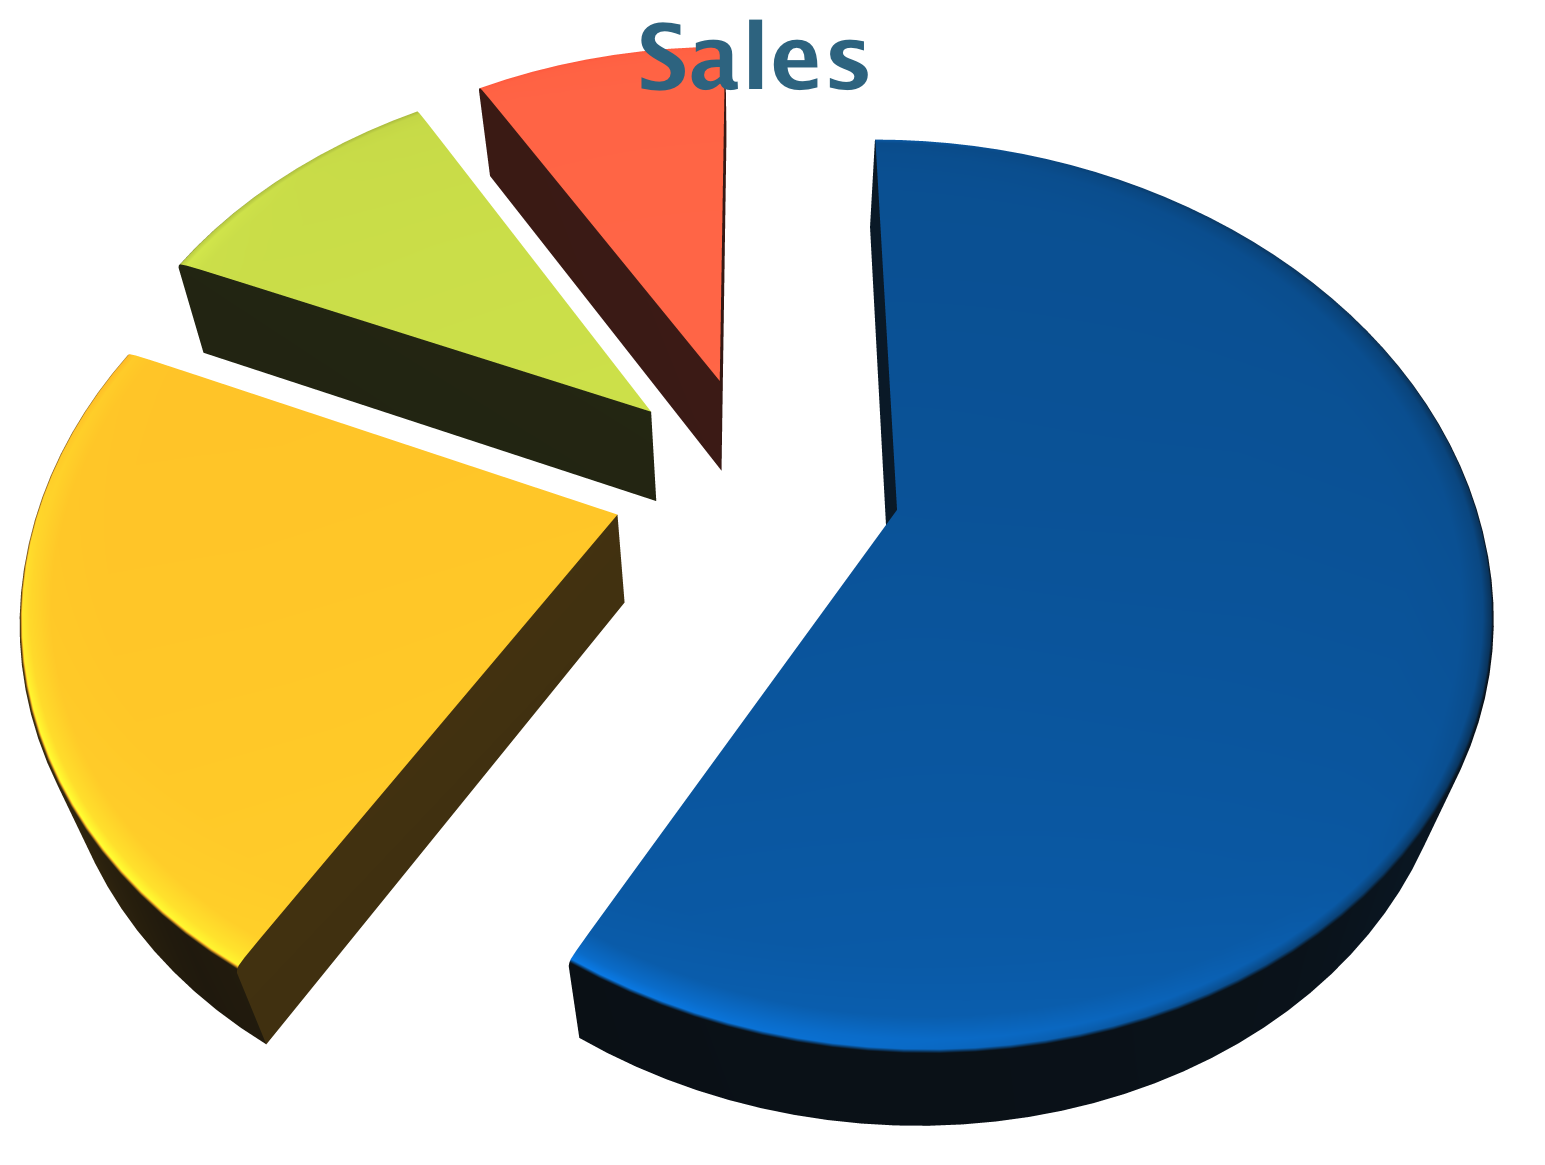
\includegraphics[width=0.4\textwidth]{chart}
\caption{\label{fig:your-figure}Caption goes here.}
\end{figure}
\end{frame}

\begin{frame}
\frametitle{Text in Two Columns}

\begin{columns}[T]

\begin{column}{0.48\textwidth}
\small
Lorem ipsum dolor sit amet, consectetur adipiscing elit. Fusce sit amet massa in dolor pellentesque tempor. Integer nunc. 
\end{column}

\begin{column}{0.48\textwidth}
\begin{itemize}
\item First bullet goes here
  \begin{itemize}
  \item Secondary bullet goes here
    \begin{itemize}
    \item Tertiary bullet goes here
    \end{itemize}
  \end{itemize}
\end{itemize}
\end{column}

\end{columns}
\end{frame}


\end{document}
